\documentclass[a4paper,11pt]{article}
\usepackage[margin=2.5cm]{geometry} % Make more reasonable margins in document
\usepackage[parfill]{parskip}  % Remove LaTeX indents, and add interparagraph space
\usepackage[utf8]{inputenc}
\usepackage[english]{babel}

\usepackage{enumitem} % Enumerations met letters in de plaats van cijfers

%%%%%%%%%%%%
%%% MATH %%%
%%%%%%%%%%%%
\usepackage{mathtools}
\usepackage{amssymb}
\usepackage[output-decimal-marker={,}]{siunitx}
\newcommand\Log[1]{ \mathop{{}^{#1}\mathrm{log}} }
\DeclarePairedDelimiterX{\norm}[1]{\lVert}{\rVert}{#1}

% https://tex.stackexchange.com/questions/94032/fancy-tables-in-latex
\usepackage[table]{xcolor}
\usepackage{booktabs}

\usepackage[utf8]{inputenc}
\usepackage{pdfpages}

%Visuals
\usepackage{graphicx}
\usepackage{subcaption}
\usepackage[colorlinks,allcolors=violet]{hyperref}
\usepackage{url}
\usepackage[T1]{fontenc}
\usepackage{lmodern} 
\usepackage{algorithm}
\floatname{algorithm}{Algoritme}
\usepackage{algorithmic}
\usepackage{courier}
\usepackage{wrapfig}
\usepackage[export]{adjustbox}
\usepackage{wasysym}

%Figures
\usepackage{pgfplots}
\pgfplotsset{compat=newest}
%% the following commands are needed for some matlab2tikz features
\usetikzlibrary{plotmarks}
\usetikzlibrary{arrows.meta}
\usepgfplotslibrary{patchplots}
\usepackage{grffile}
\usepackage{amsmath}
\usepackage{caption}
\usepackage{float}
\usepackage{cleveref}
\usepackage{multirow}
\usepackage{titlesec}
\usepackage{listings}

\usepackage{multicol}
\usepackage{tikz}
\lstset{
	language=Matlab,
	%    basicstyle={\ttfamily \small},
	basicstyle={\ttfamily \small},
	%    keywordstyle=\underline,
	numberstyle={\footnotesize},
	%    morekeywords={ones,mod,isprime,inline,unique,factor,@},
	%    flexiblecolumns=false,
	%    emph={gamma,beta},
	%    emphstyle=,
	columns=fullflexible,
	%    columns=flexible,
	%    commentstyle={\slshape},
	%    commentstyle={\normalfont},
	commentstyle={\ttfamily},
	stringstyle={\ttfamily \bfseries},
	showstringspaces=false,
	%    indent=1em,
	%    xleftmargin=0.5em,
	breaklines=false,
	%    frame={l},
	captionpos={t},
	upquote=true, % such that we can copy-paste the code...
	%    mathescape=true,
	%    frame=single,     % boxed in a single line
	%    frame=L,          % double line on the left
	%    frame=l,          % single line on the left
}

\newcommand*\circled[1]{\tikz[baseline=(char.base)]{
            \node[shape=circle,draw,inner sep=0.1pt] (char) {#1};}}
\newcommand{\note}[1]{{\colorbox{yellow!40!white}{#1}}}
\titleformat{\section}
{\normalfont\Large\bfseries}{\boxed{\text{Assignment \thesection}}}{1em}{}

\setlength{\pdfpageheight}{11in}


\title{Nonlinear Systems \\[1ex]
    \Large \textsc{Assignments}}
\author{Elias Wils}
\date{\today}

\begin{document}

\maketitle
\newpage
\tableofcontents

\newpage
\section{Stability of equilibrium points and \\bifurcations}    
\subsection{A simple population model}
\paragraph{Question 1}\: The position and number of equilibrium points depends on the value of $\alpha$ and $\beta$.
In \Cref{tbeq1} the different possible cases are listed together with information about the equilibrium points.
When looking at the graph of $\dot{N}$ against $N$, a negative parabola can be observed, intersecting the $N$-axis in two points.
When solving the quadratic equation for $\dot{N}=0$ with $\alpha$ and $\beta$ as unknown parameters, expressions shown in (1) and \eqref{eqN2} for
the equilibrium points ensue.
\begin{align}
	N_1 &= 0\\
	N_2 &= \frac{K(\alpha-\beta)}{\alpha}
	\label{eqN2}
\end{align}
\begin{table}[H]
	\centering
	\begin{tabular}{|c|c|c|}
	\hline
	$\alpha<\beta$ & $\alpha>\beta$ & $\alpha=\beta$\\
	\hline
	$N_1$ is stable (\CIRCLE) & $N_1$ is unstable (\Circle) & $N_1=N_2$\\
	$N_2$ is unstable (\Circle) & $N_2$ is stable (\CIRCLE) & half stable equilibrium point (\RIGHTcircle)\\
	\hline
	\end{tabular}
	\captionsetup{width=0.9\textwidth}
	\caption{Summary of the characteristics of the equilibrium points for different cases of $\alpha$ and $\beta$. }
	\label{tbeq1}
\end{table}
The type of bifurcation that occurs here is called transcritical. A qualitative representation of this bifurcation can be seen in 
\Cref{fig:trbif}, with the different cases in the same order as in \Cref{tbeq1}. Here the x-axis represents $N$, and the 
y-axis represents $\dot{N}$
\begin{figure}[H]
	\centering
	\makebox[\textwidth][c]{
	\begin{subfigure}{0.45\linewidth}
		\centering
		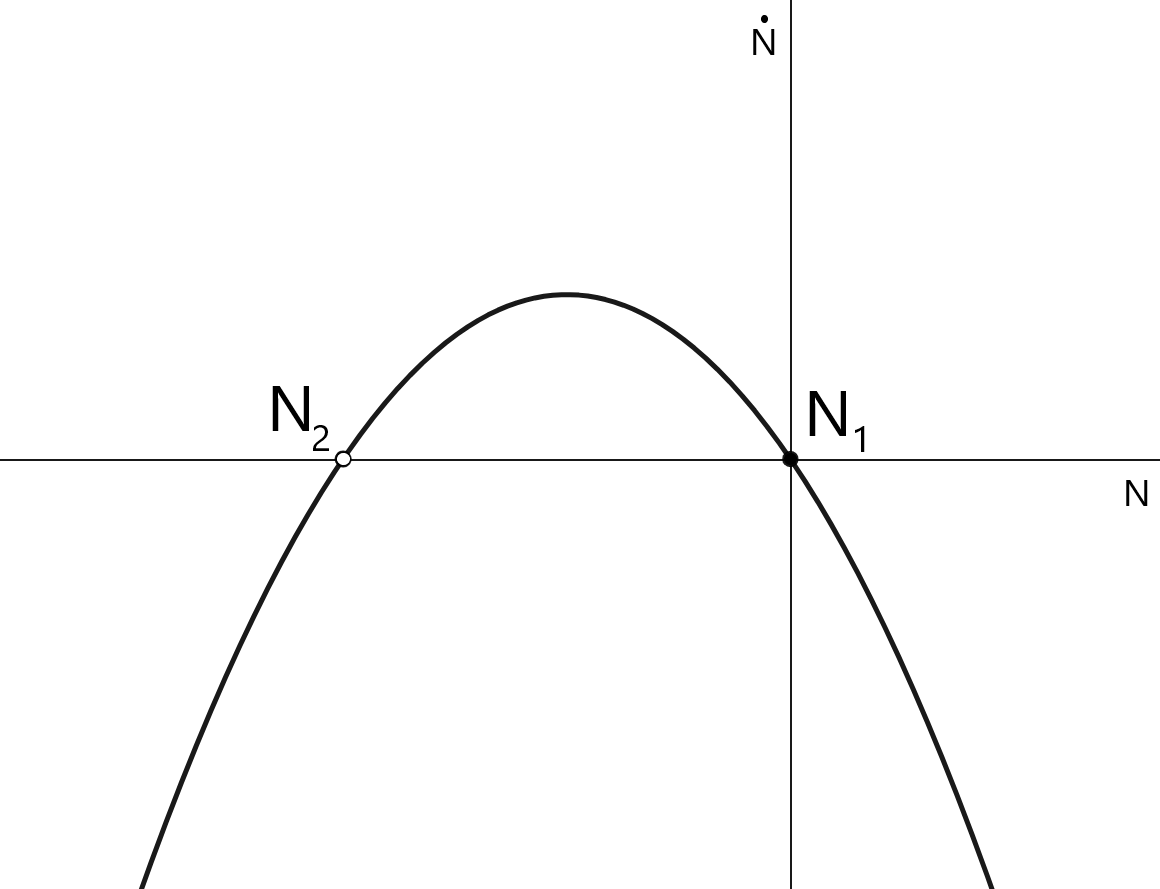
\includegraphics[width=\textwidth]{altb.png}
		\caption{$\alpha<\beta$}
	\end{subfigure}\hfill
	\begin{subfigure}{0.45\linewidth}
		\centering
		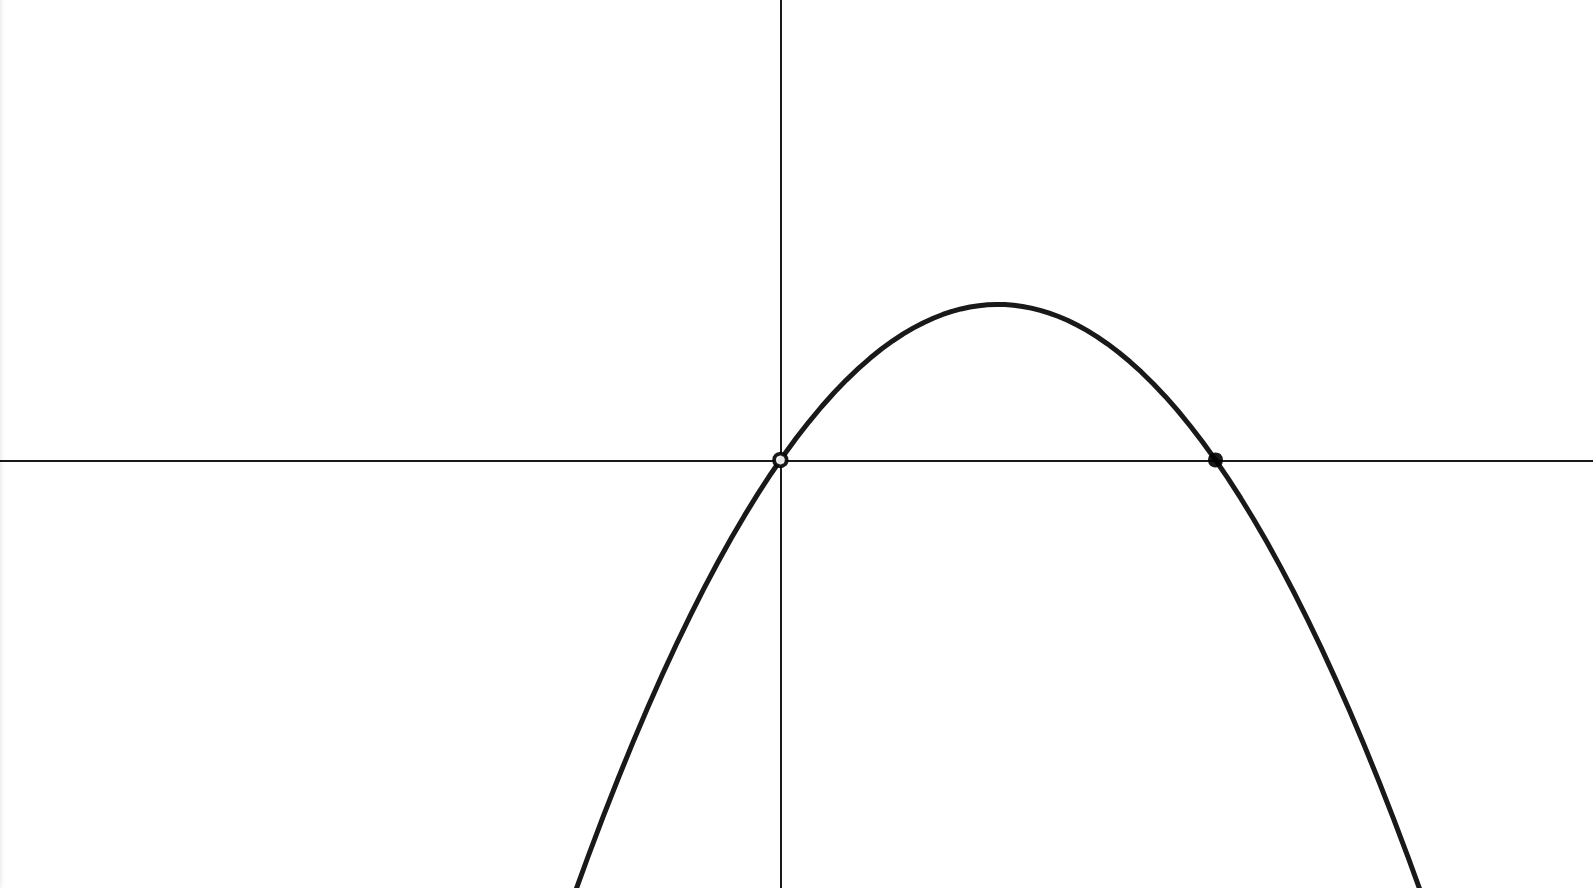
\includegraphics[width=\textwidth]{agtb.png}
		\caption{$\alpha>\beta$}
	\end{subfigure}
	\begin{subfigure}{0.45\linewidth}
		\centering
		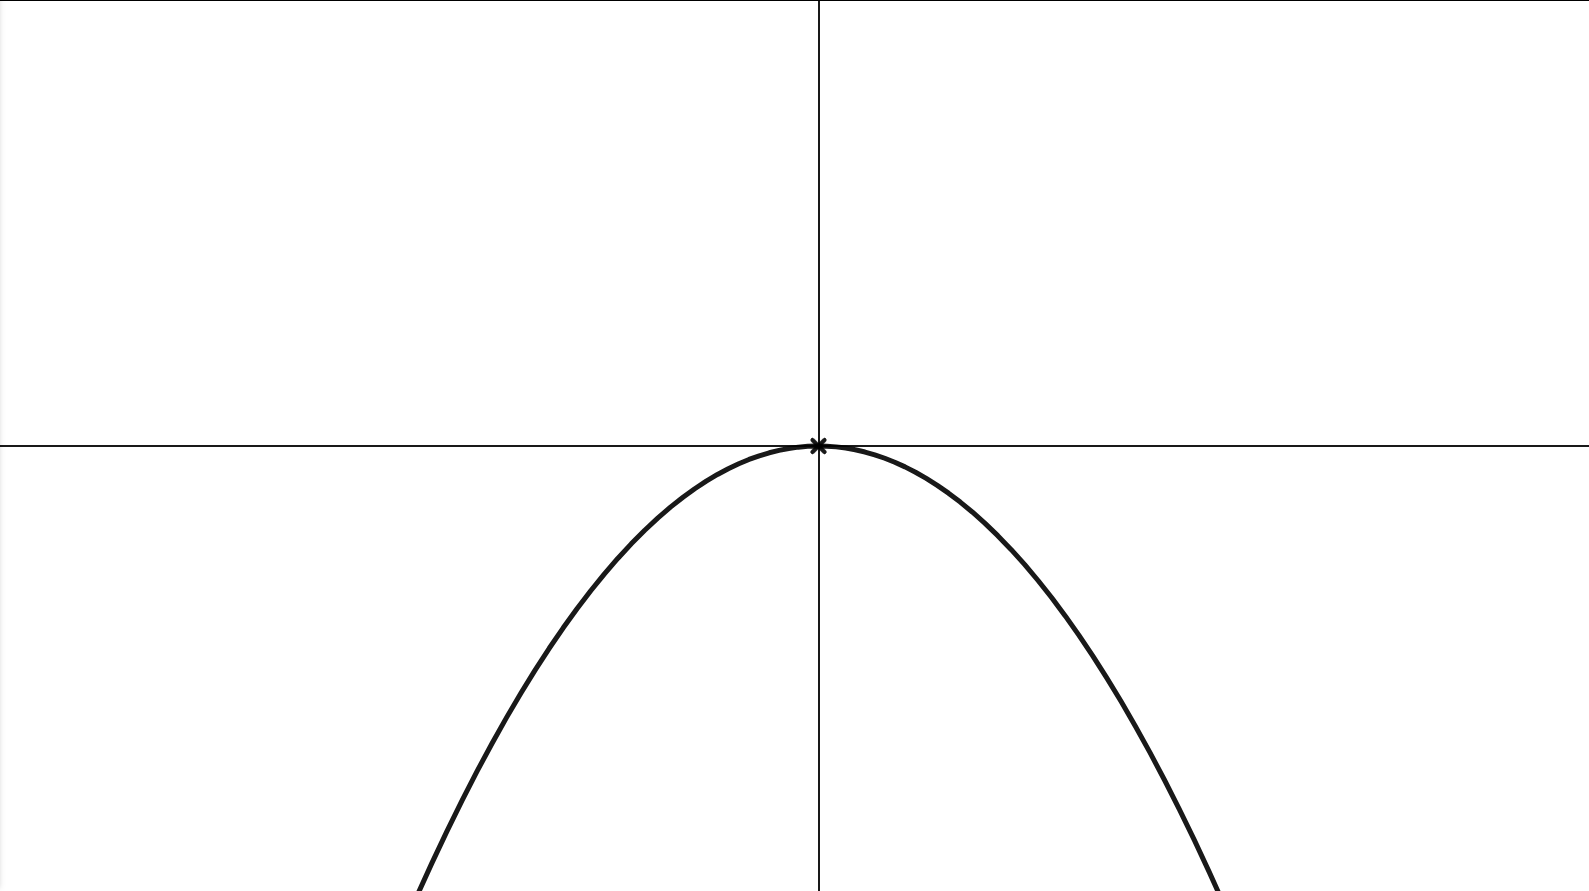
\includegraphics[width=\textwidth]{aisb.png}
		\caption{$\alpha=\beta$}
	\end{subfigure}
	}
	\caption{Qualitative plot of $\dot{N}$ against N for the different cases for $\alpha$ and $\beta$.}
	\label{fig:trbif}
\end{figure}
\paragraph{Question 2}\: For the practical example described here, the solution for $t\rightarrow\inf$ will converge to one 
of the equilibrium points. As $\alpha>\beta$, the second case in \Cref{tbeq1} is applicable. The only stable equilibrium point
is $N_2=\frac{K(\alpha-\beta)}{\alpha}=10\:470\:086$. Thus, with the parameters declared in the assignment text,
the number of inhabitants will converge towards the stable equilibrium $N_2$, which is $10\:470\:086$ here, as 
$t\rightarrow\infty$.\\

\subsection{Gene control model}
\paragraph{Question 1}\: When taking the repression rate $r=0$, only one fixed point is visible. 
The system equations become:
\begin{equation*}
	\begin{cases}
		 \dot{x}=\frac{\alpha_1}{2}-x\\
		 \dot{y}=\frac{\alpha_2}{2}-y
	\end{cases}
\end{equation*}
The only fixed point is $\left(\frac{\alpha_1}{2}, \frac{\alpha_2}{2}\right)$. We can classify fixed points
of a 2-dimensional system by analyzing the system matrix. As this system is nonlinear The Jacobian is taken 
as an approximation of this system matrix. Then the system becomes linear and an appropriate stability analysis
can be done. Below the computations are first done for the general case, whereafter $r=0$ is filled in.
The Jacobian of this nonlinear system becomes:
\begin{equation*}
	J=
	\begin{bmatrix}
		-1 & -\frac{\alpha_1ry^{r-1}}{(y^r+1)^2}\\
		-\frac{\alpha_2rx^{r-1}}{(x^r+1)^2} & -1
	\end{bmatrix}=
	\begin{bmatrix}
		-1 & 0\\
		0 & -1
	\end{bmatrix}
\end{equation*}
The trace $\tau$ of this matrix is $-2$ and the determinant $\Delta$ is:
\begin{equation*}
	\Delta=1-\frac{\alpha_1\alpha_2r^2x^{r-1}y^{r-1}}{(x^r+1)^2(y^r+1)^2}=1
\end{equation*}
In the Strogatz book there is summarized how fixed points can be classified through
$\tau$ and $\Delta$. Here $\tau<0$ and $\Delta>0$, and $\tau^2-4\Delta=0$. This means that this fixed
point is a \textbf{degenerate node}. It lies on the border between nodes and spirals, and it means that the 
eigenspace corresponding to the only eigenvalue is one-dimensional.
\paragraph{Question 2}\: $\alpha_1=\alpha_2=2$ and $r>0$.
\vspace{-5	mm}
\paragraph{i.}\: An obvious fixed point here is $(1, 1)$, and this is verified by \texttt{PPLANE},
as seen in \Cref{fig:pp1}, where a value of $r=1$ is used. 
\vspace{-5mm}
\paragraph{ii.}\: When studying the stability, there can again be made use of the Jacobian derived earlier and
fill in the given values for the parameters and $(x,y)=(1,1)$.
\begin{equation*}
	J=
	\begin{bmatrix}
		-1 & -\frac{\alpha_1ry^{r-1}}{(y^r+1)^2}\\
		-\frac{\alpha_2rx^{r-1}}{(x^r+1)^2} & -1
	\end{bmatrix}=
	\begin{bmatrix}
		-1 & -\frac{r}{2}\\
		-\frac{r}{2} & -1
	\end{bmatrix}
\end{equation*}
The expression for the determinant then becomes:
\begin{equation*}
	\Delta=1-\frac{\alpha_1\alpha_2r^2x^{r-1}y^{r-1}}{(x^r+1)^2(y^r+1)^2}=1-\frac{r^2}{4}
\end{equation*}
The trace $\tau$ stays -2. For $0< r< 2$, $\tau<0$ and $\Delta>0$ just as in Question 1.
However, now $\tau^2-4\Delta>0$, so for this range for $r$ $(1,1)$ is a stable node.\\ The special case
where $r=0$ is worked out in Question 1, then $(1,1)$ is a degenerate node. \\
Then also $r=2$ deviates from the rest. The determinant $\Delta$ then becomes zero, which means that one
of the eigenvalues is zero as the Jacobian becomes a matrix of just $-1$s. When $r$ exceeds 2, the determinant
$\Delta$ becomes negative, which means a saddle node is established.\\
These findings are summarized in \Cref{tbeq2}.
\begin{table}[H]
	\centering
	\begin{tabular}{|c|c|c|c|}
	\hline
	$r=0$ & $0<r<2$ & $r=2$ & $r>2$\\
	\hline
	$\tau=-2<0$ & $\tau=-2<0$ & $\tau=-2<0$ & $\tau=-2<0$\\
	$\Delta=1>0$ & $\Delta\in(0,1)>0$ & $\Delta=0$ & $\Delta<0$\\
	$\tau^2-4\Delta=0$ & $\tau^2-4\Delta\in(0,4)>0$ & $\tau^2-4\Delta=4>0$ & $/$\\
	degenerate node & stable node & stable line of nodes & saddle node\\
	\hline
	\end{tabular}
	\captionsetup{width=0.9\textwidth}
	\caption{Summary of the characteristics of the fixed point $(1,1)$ for $0\leq r\leq2$.}
	\label{tbeq2}
\end{table}
\vspace{-5mm}
The phase portraits for these cases are shown in \Cref{fig:pp1}, as requested in \textbf{iv}.
\vspace{-3mm}
\paragraph{iii.}\: There can be noticed that a bifurcation occurs when $r$ crosses the value 2. This bifurcation is a 
supercritical pitchfork bifurcation, because when $r>2$, a pair of stable equilibrium points appear symmetrically w.r.t. the fixed point $(1,1)$.
This fixed point $(1,1)$ is stable when $0<r<2$ and becomes unstable when $r>2$ as it becomes a saddle node.
These types of bifurcations occur in systems where there is some sort of symmetry present, as is the case here.
The two system equations are exactly the same, apart from the fact that $x$ and $y$ are interchanged. This also causes the 
Jacobian to be almost symmetrical, apart from the interchanged $x$ and $y$ again.\\
This is also seen when computing the phase plane numerically with \texttt{PPLANE}. Once $r$ exceeds 2, 
two more fixed points arise symmetrical w.r.t. the original fixed point $(1,1)$.

\paragraph{iv.}\: The phase portraits for the different cases of $r$ listed in \Cref{tbeq2} are shown in \Cref{fig:pp}.
\begin{figure}[H]
	\centering
	\makebox[\textwidth][c]{
	\begin{subfigure}[b]{0.5\textwidth}
		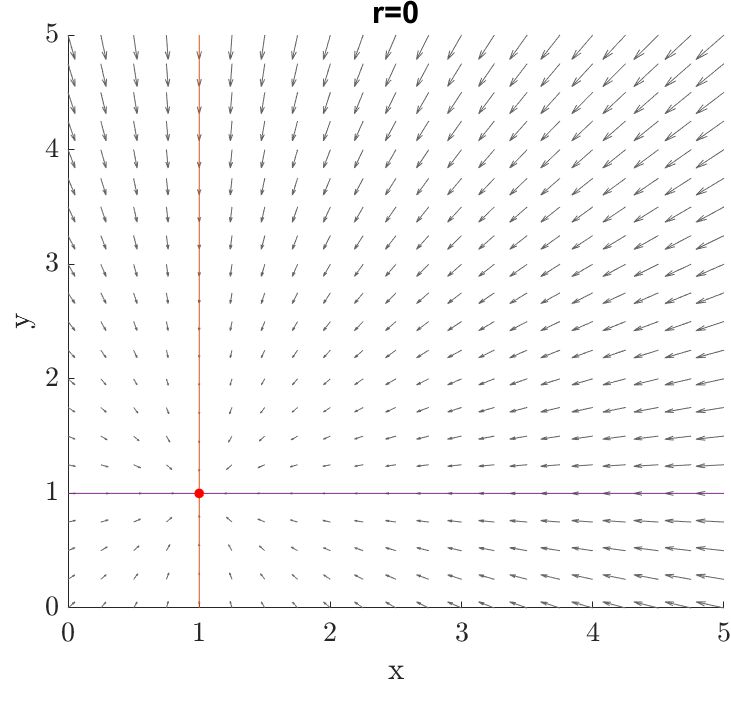
\includegraphics[width=\textwidth]{r0}
		\caption{Phase portrait for $r=0$.}
		\label{fig:r0} 
	\end{subfigure}

	\begin{subfigure}[b]{0.5\textwidth}
		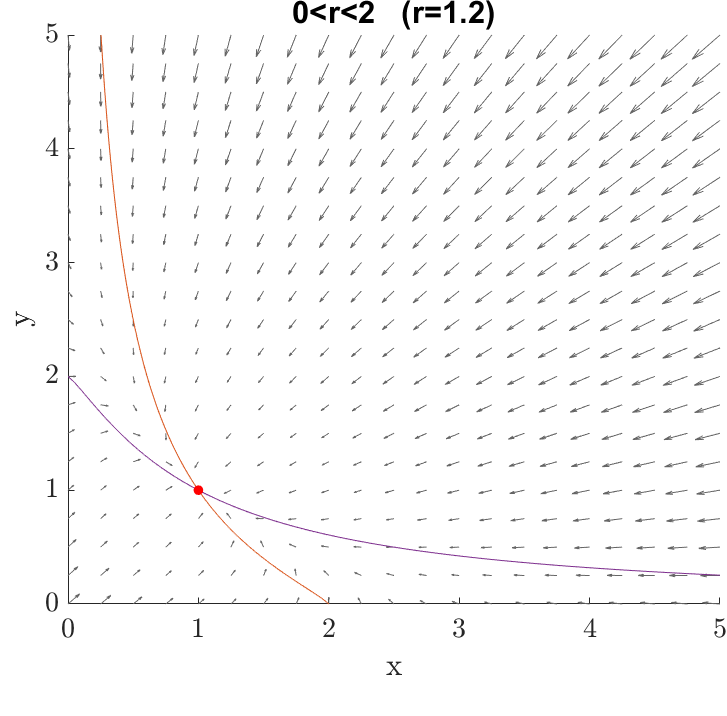
\includegraphics[width=\textwidth]{0r2.png}
		\caption{Phase portrait for $r=1.2$.}
		\label{fig:0r2}
	\end{subfigure}
	}
	\makebox[\textwidth][c]{
	\begin{subfigure}[b]{0.5\textwidth}
		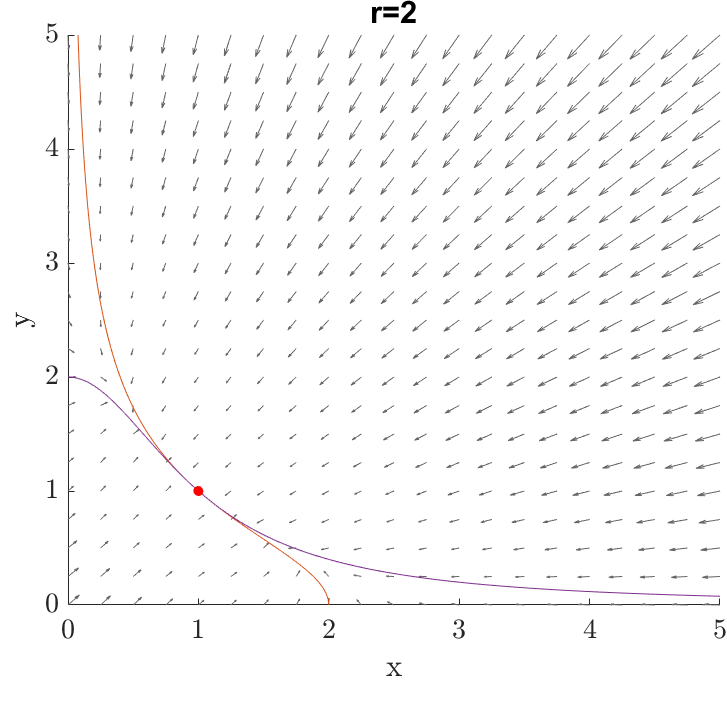
\includegraphics[width=\textwidth]{r2}
		\caption{Phase portrait for $r=2$.}
		\label{fig:r2} 
		\end{subfigure}
		
		\begin{subfigure}[b]{0.5\textwidth}
		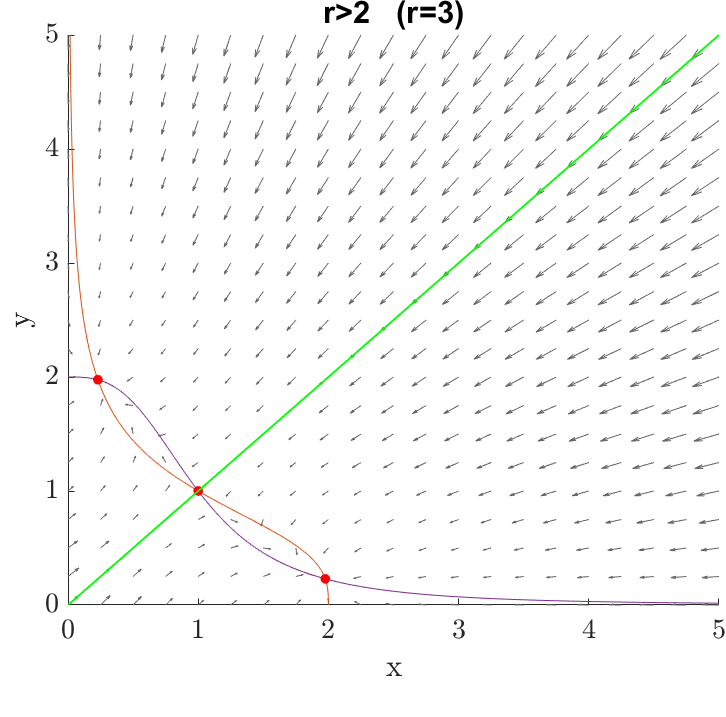
\includegraphics[width=\textwidth]{rgt2.png}
		\caption{Phase portrait for $r=3$.}
		\label{fig:rgt2}
		\end{subfigure}
	}
	\label{fig:pp1}
	\caption{Phase portraits of the given system for the qualitatively different phase portraits when varying $r$.}
\end{figure}
The bifurcation that occurs here is a supercritical pitchfork bifurcation, and a qualitative sketch of the bifurcation diagram of
either $x$ or $y$ is shown in \Cref{fig:bif}.
\begin{figure}
	\centering
	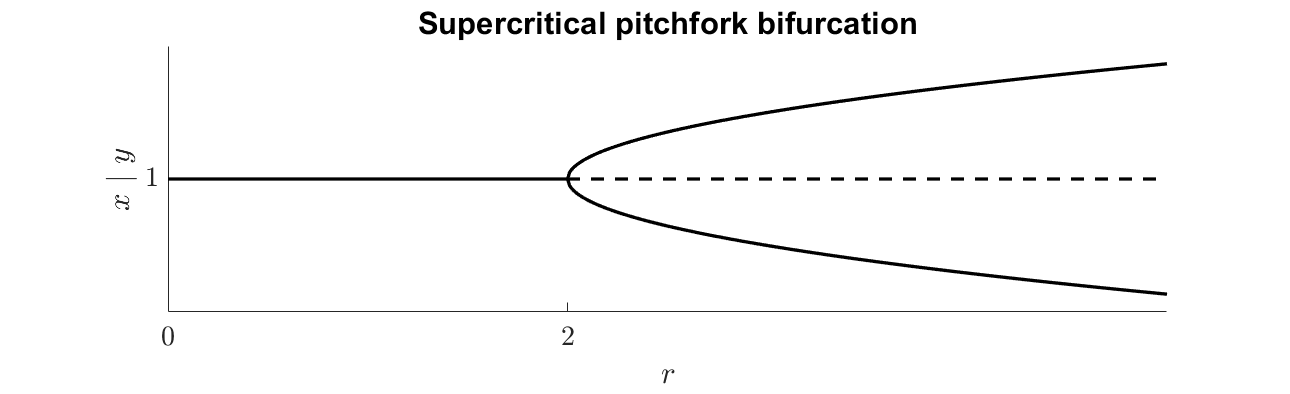
\includegraphics[width=0.9\textwidth]{suppit.png}
	\caption{Qualitative bifurcation diagram of the supercritical pitchfork bifurcation.}
	\label{fig:bif} 
\end{figure}
\end{document}

\section{Imperfect bifurcations}
\subsection{Gene control revisited}
The accurate bifurcation diagram using \texttt{COCO} can be found in \Cref{fig:bif1}. The diagram for both
$x$ and $y$ in function of $r$ is plotted, as the diagram 3-dimensional.
\begin{figure}
	\centering
	\makebox[\textwidth][c]{
	\begin{subfigure}[b]{0.5\textwidth}
		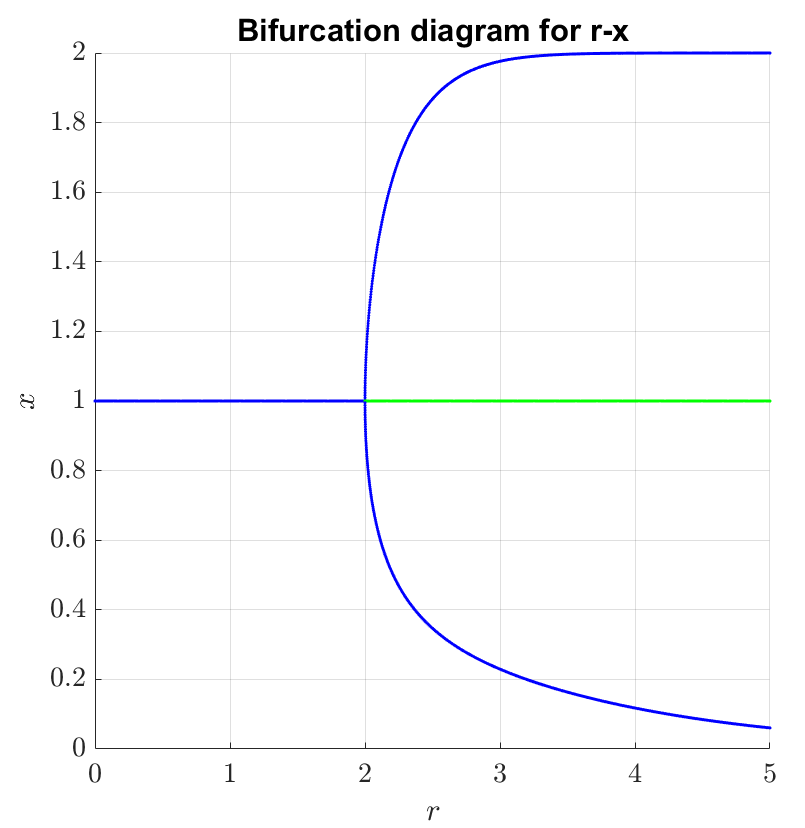
\includegraphics[width=\textwidth]{bif1x.png}
		\caption{Pitchfork for $r$ and $x$.}
		\label{fig:bif1x} 
	\end{subfigure}

	\begin{subfigure}[b]{0.5\textwidth}
		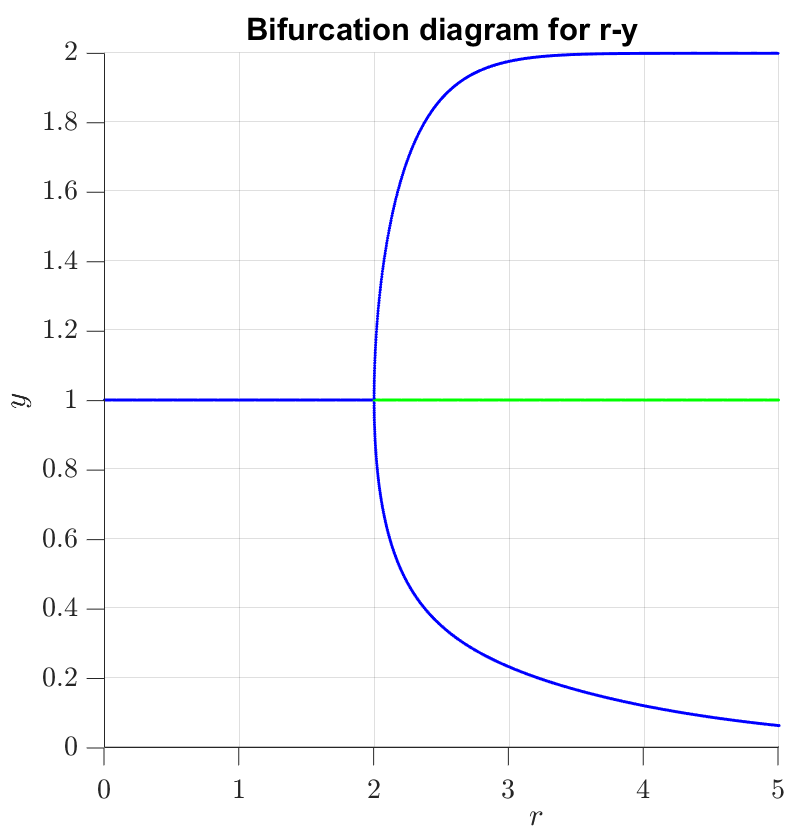
\includegraphics[width=\textwidth]{bif1y.png}
		\caption{Pitchfork for $r$ and $y$.}
		\label{fig:bif1y}
	\end{subfigure}
	}
	\label{fig:bif1}
	\caption{Bifurcation diagram of the supercritical pitchfork bifurcation in both $x$ and $y$.}
\end{figure}